% ****** Start of file .tex ******
%
%   This file is based on apssamp.tex, part of the APS files in the REVTeX 4.1 distribution.
%   Version 4.1r of REVTeX, August 2010
%
%   Copyright (c) 2009, 2010 The American Physical Society.
%   Samuel Balula, Pedro Ribeiro, Luís Macedo, Eduardo Neto 2013
%   See the REVTeX 4 README file for restrictions and more information.
%
% TeX'ing this file requires that you have AMS-LaTeX 2.0 installed
% as well as the rest of the prerequisites for REVTeX 4.1
%
% See the REVTeX 4 README file
% It also requires running BibTeX. The commands are as follows:
%
%  1)  latex filename.tex
%  2)  bibtex filename
%  3)  latex filename.tex
%  4)  latex filename.tex

\documentclass[%
  reprint,
  %superscriptaddress,
  %groupedaddress,
  %unsortedaddress,
  %runinaddress,
  %frontmatterverbose, 
  %preprint,
  %showpacs,preprintnumbers,
  nofootinbib,
  %nobibnotes,
  %bibnotes,
  amsmath,amssymb,
  aps,
  %pra,
  %prb,
  %rmp,
  %prstab,
  %prstper,
  %floatfix,
  10pt,
  a4paper
]{revtex4-1}



\usepackage{facil}                      % Pacote pessoal
\usepackage{verbatim}                   % Apresentação de código
\usepackage{graphicx}                   % Include figure files
\usepackage{dcolumn}                    % Align table columns on decimal point
\usepackage{bm}                         % bold math
\usepackage[latin1,utf8]{inputenc}      % Tipos de caracteres
\usepackage[portuges]{babel}            % Português
\usepackage{indentfirst}                % Identação da primeira linha
\usepackage{hyperref}                   % add hypertext capabilities
\usepackage{float}                      %Fixar imagens
\usepackage{multirow}
%\usepackage[mathlines]{lineno}          % Enable numbering of text and display math
%\linenumbers\relax                      % Commence numbering lines
%\usepackage[compact]{titlesec}

\usepackage[%showframe,%Uncomment any one of the following lines to test 
%%scale=0.7, marginratio={1:1, 2:3}, ignoreall, % default settings
%%text={7in,10in},centering,
margin=0.5in,        %diminuir margens
%total={6.5in,8.75in}, top=1.2in, left=0.9in, 
includefoot
%height=10in,a5paper,hmargin={3cm,0.8in},
]{geometry}

\begin{document}
\preprint{APS/123-QED}
%\captionsetup[table]{font=small,skip=0pt}
%\captionsetup[figure]{font=small,skip=0pt}
%\titlespacing{\section}{0pt}{*0}{*0}            %Poupar espaço
%\titlespacing{\subsection}{0pt}{*0}{*0}
%\titlespacing{\subsubsection}{0pt}{*0}{*0}


% % % % % % % % % % % % % % % % % % % % % % % % % % % % % % % % % % % % % % % % 
%%%%%%%%%%%%%%%%%%%%%%%%%%%%%%%%%% Início %%%%%%%%%%%%%%%%%%%%%%%%%%%%%%%%%%%%%%
% % % % % % % % % % % % % % % % % % % % % % % % % % % % % % % % % % % % % % % %
 

\title{Andar final de amplificação em classe A\\
com transistores bipolares 2n3055}
\thanks{}

\author{Pedro Ribeiro}%
\email{73221, pedro.q.ribeiro@tecnico.ulisboa.pt}
\author{Luis Macedo}%
\email{73633, luis.macedo@tecnico.ulisboa.pt}
\author{Samuel Balula}%
\email{72735, samuel.balula@tecnico.ulisboa.pt}

\affiliation{
  Instituto Superior Técnico\\
  Mestrado em Engenharia Física Tecnológica\\
  Complementos de Electrónica
}

%\collaboration{Grupo 57}

\date{\today}

%%%%%%%%%%%%%%%%%%%%%%%%%%%%%%%%%% Abstract %%%%%%%%%%%%%%%%%%%%%%%%%%%%%%%%%%%%
\begin{abstract}
Neste trabalho laboratorial é montado um andar de saída em classe A, usando transístores bipolares 2n3055.
Medem-se, calculam-se e determinam-se com recurso a uma simulação em spice as correntes, tensões e potências com o circuito no ponto de funcionamento em repouso bem como com sinais periódicos de diferentes frequências.
Determinam-se a função de transferência, característica de corrente, impedâncias de entrada e saída e banda passante.
RESULTADOS!!!!!!!!!!!!!!!!!!!!!!!!!!!!!!!!!!!!!!!!!!!!!!!!

\end{abstract}
\maketitle


%%%%%%%%%%%%%%%%%%%%%%%%%%%%%%%%%% Introdução %%%%%%%%%%%%%%%%%%%%%%%%%%%%%%%%%%
\section{Introdução}
\label{s:intro}
%Situar o problema, incluir fórmulas.
%Quem lê o relatório deve conseguir perceber exatamente o que foi feito.

Um andar de saída em classe A é um tipo de amplificador que permite aumentar a potência de um sinal e fornecê-lo a uma carga. Nesta tipologia o dispositivo está em condução em todo o ciclo do sinal, o que resulta numa baixa distorção do sinal mas uma baixa eficiência.

\fig[.30]{../img/esquematico.png}{Circuito implementado no laboratório}

Neste trabalho laboratorial implentou-se o circuito representado na \rfig{../img/esquematico.png} e que se descreve em maior detalhe em \ref{s:expreal}

\subsection{Ponto de funcionamento em repouso}
Para o cálculo do ponto de funcionamento em repouso utilizaram-se as seguintes relações para os transístores:
\eq[r0]{
\begin{cases} i_C = \beta_f i_B \\
i_E = \lr{\beta_f +1} i_B \\
i_E = \frac{\beta_f+1}{\beta_f} i_C
\end{cases}}
\eq[r1]{i_E	= I_{ES} \lr{e^{\frac{v_{BE}}{\eta V_T}}-1} \approx I_{ES} \lr{e^{\frac{v_{BE}}{\eta V_T}}}}
\eq[i0]{v_{BE} = \eta V_T \log\lr{\frac{i_E}{i_{ES}}+1} = \eta V_T \log\lr{\frac{i_C}{i_{ES}}\frac{\beta_f+1}{\beta_f}+1}}

Analise-se o circuito de fonte de corrente, constituído pelos transístores Q2 e Q3, e pela resistência R2. Dada a simetria do circuito, as correntes e tensões nos dois transístores são iguais ($i_{B2}=i_{B3}$, $i_{C2}=i_{C3}=I$, $v_{BE1}=v_{BE3}$). Pode assim escrever-se:
\eq{i_R = i_C + i_{B2} + i_{B3} = i_C + 2 i_B}
\eq{-\frac{V_{SS}+V_{BE2}}{R_2} = \lr{\beta_f + 2} i_B = \frac{\beta_f + 2}{\beta_f} I}

Resolvendo em ordem a $v_{BE}$:
\eq[i1]{v_{BE} = -R_2 \frac{\beta_f + 2}{\beta_f} I - V_{SS}}

Igualando \eqref{i0} e \eqref{i1}:
\eq{I = - \frac{\beta_f}{\beta_f + 2}  \frac{V_{SS} + \eta V_T \log\lr{\frac{I}{i_{ES}}\frac{\beta_f+1}{\beta_f}+1}}{R_2}}

Esta é uma equação transcendente, que pode ser resolvida numericamente. Seja I a corrente fornecida por esta parte do circuito.

\subsection{Função de transferência}

Aplicando a lei dos nós ao ponto 12 do circuito:

\eq{i_{E1} = I_{R1} + I = \frac{v_0}{R_1} + I}

\eq{v_{BE} = v_i - i_B (R_g + R_3) - v_0 = v_i - \frac{i_e}{1 + \beta_f} (R_3+R_g) - v_0}

Pode assim escrever-se a característica $v_i(v_o)$:

\eq{v_i = \eta V_T \log\lr{\frac{\frac{v_0}{R_1} + I }{I_{ES}} + 1} + v_0 + \lr{\frac{v_0}{R_1} + I}\frac{R_3 + R_g}{1+\beta_f}}

Desprezando o termo +1 no argumento do logaritmo e o último termo da expressão:

\begin{equation}
v_i=v_o+\eta v_T\log \left(\frac{I+\frac{v_o}{R_1}}{I_{ES}}\right)
\end{equation}

\begin{equation}
G_v=\left(\frac{\mathrm{d}v_i}{\mathrm{d}v_o}\right)^{-1}=\left(1+\frac{\eta v_T}{I+\frac{v_o}{R_1}}\right)^{-1}\approx 1
\label{eq:g_v}
\end{equation}

Para determinar o ganho de corrente basta observar que:
\begin{equation}
\begin{cases} i_e=i_c+i_b\\ i_c=\beta_F i_b
\end{cases}
\end{equation}
E assim:
\begin{equation}
i_e=(\beta_F+1)i_b
\end{equation}
E consequentemente o ganho em corrente é dado por:
\begin{equation}
G_i=\beta_F+1
\label{eq:g_i}
\end{equation}
Para determinar a tensão máxima na saída, basta notar que quando a tensão na saída é máxima, o transístor entra na região de saturação, pelo que a sua tensão $V_{CE}$ vai ter um valor bem definido e logo:
\begin{equation}
V_{o_{max}}=V_{CC}-V_{{CE}_{sat}}
\label{eq:sat}
\end{equation}

Para determinar a eficiência das montagens e o rendimento dos transístores, é necessário determinar a potência dissipada pelos transístores Q1 e Q2.
A potência dissipada pelo transístor Q1 é dada por:
\begin{equation}
P_{Q1}=\langle i_{c_1} V_{{CE}_1}\rangle
\end{equation}
Começa-se por determinar o factor $i_{c_1} V_{{CE}_1}$:
\begin{equation}
i_{c_1} V_{{CE}_1}=(V_{CC}-v_o)\left(I+\frac{v_o}{R_1}\right)=V_{CC}I+V_o\left(\frac{V_{CC}}{R_1}-I\right)-\frac{v_o^2}{R_1}
\end{equation}
Como $\frac{V_{CC}}{R_1}-I\approx0$, simplificando a expressão anterior e fazendo a média:
\begin{equation}
P_{Q1}=\left\langle V_{CC}I-\frac{v_o^2}{R_1} \right\rangle=V_{CC}I-\frac{(V_{CC}-V_{{CE}_sat})^2}{2R_1}
\end{equation}
Para o transístor Q2, a potência dissipada é dada por:
\begin{equation}
P_{Q2}=\langle I(v_o-V_{DD}) \rangle=IV_{DD}
\end{equation}
Estamos agora em condições de calcular a eficiência da montagem. A eficiência é dada por:
\begin{equation}
\eta=\frac{P_{R_1}}{P_{S+}+P_{S-}}
\end{equation}
$P_{S-}$ é a potência fornecida pela fonte de tensão negativa $V_{DD}$ e é dada por:
\begin{equation}
P_{S-}=V_{DD}I
\end{equation}
A potência fornecida pela fonte de tensão positiva $V_{CC}$ já não vai ser constante e vai passar a ser dada por:
\begin{equation}
P_{S+}=\langle V_{cc} i_c \rangle \approx \langle V_{cc} i_e \rangle =\left\langle V_{cc} I+\frac{v_o}{R_1} \right\rangle \approx V_{CC}I
\end{equation}
A potência máxima fornecida à carga (interessa saber qual a potência máxima, de modo a determinar a eficiência máxima) é dada por:
\begin{equation}
P_{L}=\frac{V_{o_m}}{2R_1}
\end{equation}
Com estas fórmulas para a potência é agora possível determinar a eficiência máxima, fazendo:
\begin{equation}
\eta=\frac{1}{4}\frac{v_{o_m}}{IR_1}\frac{v_{o_m}}{V_{CC}}\approx\frac{1}{4}=25\%
\end{equation}

\subsection{Impedâncias de entrada e saída}

De modo a determinar a impedância de entrada do circuito mede-se a corrente e a tensão de entrada utilizando um multímetro e determina-se a impedância a partir da equação \ref{eq:impedanciaentrada}.
\begin{equation}
Z_{in}=\frac{V_{in}}{I_{in}}
\label{eq:impedanciaentrada}
\end{equation}
Para determinar a impedância de saída do circuito utilizam-se duas cargas diferentes e considera-se que o circuito é linear de modo a poder ser possível considerar um equivalente de Thévenin. A impedância de saída é obtida através da equação \ref{eq:impedanciasaida}.
\begin{equation}
Z_{out}=\frac{R_1 \frac{dV_0}{dR_1}}{\frac{V_0}{R_1}-\frac{dV_0}{dR_1}}
\label{eq:impedanciasaida}
\end{equation}

É também pretendido verificar a resposta em frequência do circuito e para tal varia-se a frequência do sinal de entrada e apresenta-se o gráfico de $\frac{i_0}{i_i} (dB)$ em função de $log(f)$. De modo a saber as correntes de entrada e saída medem-se as tensões respetivas e utiliza-se $I=\frac{V}{R}$. Determina-se ainda o limite superior da banda passante a $-3dB$ partir da intersecção dessa recta com o gráfico já referido. 

%%%%%%%%%%%%%%%%%%%%%%%%%%%% Experiência realizada %%%%%%%%%%%%%%%%%%%%%%%%%%%%%
\section{Experiência Realizada}
\label{s:expreal}
%Incluir diagrama de blocos da montagem
De acordo com as instruções do guia, implementou-se o circuito da \rfig{../img/esquematico.png}. Apresentam-se na tabela \ref{partlist} os componentes utilizados.
Efetuaram-se as medições:


\tabela[partlist]{Lista dos componentes utilizados}{lrrr}{
	Descrição		&Modelo/Valor		&Qt.			&Referência	\\ \hline
	Transístor J. Bipolar	&2n3055			&3			&Q1,Q2,Q3	\\
	Gerador de Sinais	&			&1			&		\\
	Resistência de potência	&10$\Omega$		&2			&R2,R3	\\
	Reóstato de potência	&12$\Omega$		&1			&R1
}


%%%%%%%%%%%%%%%%%%%%%%%%%%%%%%%% Resultados %%%%%%%%%%%%%%%%%%%%%%%%%%%%%%%%%%%%
\section{Resultados}
\label{s:resul}

%incluir tabelas. Excesso de dados => grafico com valores mais significativos

\subsection{Ponto de funcionamento em repouso}
Apresentam-se na tabela \ref{PFR} os valores de tensões e correntes relevantes medidos experimentalmente, calculados teoricamente e obtidos na simulação.\footnote{Para facilidade de leitura apresentam-se apenas os valores que foram medidos diretamente. As restantes correntes e tensões que não estão apresentadas podem ser calculadas por aplicação direta da lei de Ohm}

\tabela[PFR]{Valores de corrente e tensão, conforme legenda da \rfig{../esquematico.png}}{llll}{
ID	&Experimental		&Teórico	&Simulação	\\ \hline
Vdd (V)	&$8.022\pm0.01$		&$8.000$	&$8.000$	\\
Vss (V)	&$-8.006\pm0.01$	&$-8.000$	&$-8.000$	\\
10  (V)	&$-0.420\pm0.002$	&$-0.181$	&$-0.365$	\\
11  (V)	&$-0.574\pm0.001$	&$-0.218$	&$-0.438$\\
12  (V) &$-1.296\pm0.001$	&$-1.639$	&$-1.149$\\
13  (V) &$-7.253\pm0.001$	&$-6.454$	&$-7.275$\\ \hline
20  (A) &$1.12\pm0.02$		&$0.468$	&$0.724$\\
21  (A) &$1.88\pm0.02$		&$1.281$	&$1.574$\\
22  (A) &$1.23\pm0.02$		&$0.636$	&$0.847$\\
R1  ($\Omega$)	&$10\pm1$	&$10$		&$10$

}

\tabela[Potdiss]{Potências dissipadas no PFR, valores em Watt}{llll}{
ID	&Experimental		&Teórico	&Simulação	\\ \hline
$Vdd$		&$-9.06\pm0.17$		&$-3.74$	&$-5.79$ \\
$Vss$		&$-15.05\pm0.18$	&$-10.24$	&$-12.59$\\
Ger. sinais	&$-0.0064\pm0.0001$	&$-0.0007$	&$-0.0026$\\
$R_1$		&$0.1680\pm0.0003$	&$0.2686$	&$0.1320$\\
$R_2$		&$5.2606\pm0.0014$	&$4.1654$	&$5.2926$\\
$R_3$		&$0.0024\pm0.0001$	&$0.0001$	&$0.0005$\\
$Q_1$		&$10.53\pm0.20$		&$4.5111$	&$6.6239$\\
$Q_2$		&$8.25\pm0.15$		&$4.04$		&$5.80$\\
$Q_3$		&$0.489\pm0.037$	&$1.00$		&$0.527$\\ \hline
Somatório	&$0.580\pm0.858$	&$-0.005$	&$-0.003$


}


\subsection{Função de transferência}
Neste ponto obtiveram-se as relações entre as correntes e as tensões de entrada e saída da montage utilizada. Foi utilizado o osciloscópio para medir tanto a tensão de entrada como a de saída do circuito, obtiveram-se as correntes de entrada e saída medindo a tensão aos terminais da resistência de entrada e de saída com o osciloscópio, tendo-se obtido a corrente através da lei de Ohm.\\
A relação entre tensão de entrada e saída deste circuito está apresentada na figura \ref{fig:v_rel}. Para determinar o ganho da montagem utilizada, realizou-se também um ajuste linear:
\begin{equation}
y(x)=ax+b
\end{equation}
Onde a variável x é a tensão de entrada, a variável y a tensão de saída, a é o ganho e b é o desvio da origem.
\begin{figure}
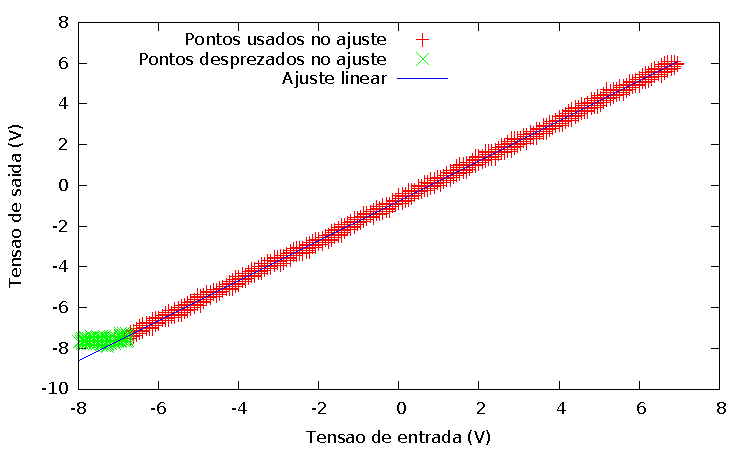
\includegraphics[width=3in]{v_rel.pdf}
\caption{Gráfico da relação entre tensão de entrada e de saída da montagem utilizada e respectivo ajuste linear. É possível observar que para valores de tensão de entrada muito negativa, começa a haver distorção.}
\label{fig:v_rel}
\end{figure}
Os resultados obtidos através do ajuste foram os seguintes: a=$G_v=0.96\pm0.01$, b=$-0.69\pm0.01$V.

Para a relação entre corrente de entrada e de saída do circuito também se realizou um ajuste linear semelhante ao realizado anteriormente para se obter o ganho de corrente, apresentado juntamente com os dados experimentais na figura \ref{fig:curr_rel}.
\begin{figure}
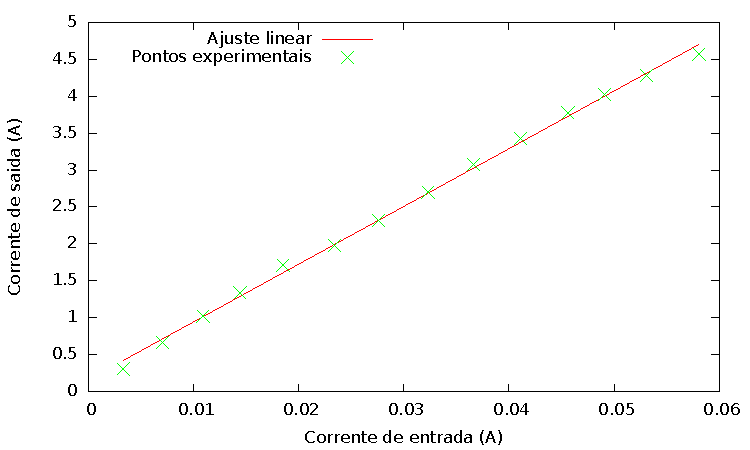
\includegraphics[width=3in]{curr_rel.pdf}
\caption{Gráfico da relação entre corrente de entrada e de saída da montagem utilizada e respectivo ajuste linear.}
\label{fig:curr_rel}
\end{figure}
Os resultados obtidos através do ajuste foram os seguintes: $a=G_i=78.12\pm1.07$, $b=0.16\pm0.04$A. 


\subsection{Potências fornecidas e dissipadas}
Os dados obtidos estão apresentados na tabela \ref{tab:fixe}, juntamente com os resultados dos cálculos para a potência dissipada e para o rendimento.
% Please add the following required packages to your document preamble:
% \usepackage{multirow}
\begin{table}[h]
\begin{tabular}{|cc|c|c|}
                                                             & \multicolumn{1}{l|}{} & $v_o=v_{o_m}$ & $v_o=\frac{v_{o_m}}{2}$ \\ \hline
$V_{CC}$ (V)                                                 & \multicolumn{1}{l|}{} & \multicolumn{2}{c|}{8.04}               \\ \hline
$V_{DD}$ (V)                                                 & \multicolumn{1}{l|}{} & \multicolumn{2}{c|}{8.01}               \\ \hline
$I(V_{CC})$ (A)                                              & \multicolumn{1}{l|}{} & \multicolumn{2}{c|}{0.6}                \\ \hline
$I(V_{DD})$ (A)                                              & \multicolumn{1}{l|}{} & \multicolumn{2}{c|}{1.3}                \\ \hline
$R_1$ ($\Omega$)                                             &                       & \multicolumn{2}{c|}{10}                 \\ \hline
\multicolumn{1}{|c|}{\multirow{2}{*}{$V_o$ (V)}}             & multímetro            & -0.95         & -0.98                   \\ \cline{2-4} 
\multicolumn{1}{|c|}{}                                       & osciloscópio          & -0.93         & -0.95                   \\ \hline
\multicolumn{1}{|c|}{\multirow{2}{*}{$P_{Q_1}$ (W)}}         & multímetro            & 5.39          & 5.41                    \\ \cline{2-4} 
\multicolumn{1}{|c|}{}                                       & osciloscópio          & 5.38          & 5.39                    \\ \hline
\multicolumn{1}{|c|}{\multirow{2}{*}{$P_{Q_2}$ (W)}}         & multímetro            & 5.52          & 7.82                    \\ \cline{2-4} 
\multicolumn{1}{|c|}{}                                       & osciloscópio          & 5.52          & 7.81                    \\ \hline
\begin{tabular}[c]{@{}c@{}}Potência\\ dissipada\end{tabular} &                       & 10.89         & 13.2                    \\ \hline
\begin{tabular}[c]{@{}c@{}}Potência\\ fornecida\end{tabular} &                       & 15.24         & 15.24                   \\ \hline
Rendimento (\%)                                              &                       & 13.59         & 3.86                   
\end{tabular}
\caption{Tensões e potências dissipadas obtidas para os trasístores $Q_1$ e $Q_2$ da montagem utilizada.}
\label{tab:fixe}
\end{table}
É de notar que o rendimento obtido é bastante baixo, na ordem dos 15\% quando $v_o=v_{o_{max}}$ e na ordem dos 4\% quando $v_o=\frac{v_{o_m}}{2}$. É interessante notar que a eficiência obtida experimentalmente é bastante inferior à eficiência de 25\% obtida teoricamente. Isto deve-se ao facto de no cálculo da eficiência apenas se ter considerado as perdas nos transístores $Q_1$ e $Q_2$, quando existem outros elementos do circuito onde também existe dissipação.









\subsection{Impedâncias de entrada e saída}
Neste ponto mediram-se a tensão e corrente de entrada directamente utilizando o multímetro, de modo a determinar a impedância de entrada. Mediram-se também, utilizando duas cargas diferentes, a corrente e tensão nessas cargas, para que, a partir do equivalente de Thévenin fosse possível determinar a impedância de saída do circuito. Os resultados estão na tabela \ref{tab:impedancia}.

\begin{table}[h]
    \begin{tabular}{|l|l|}
\hline
         $ V_i (V)$	&	$0.874  \pm 0.01$		                    \\ \hline
	$I_i (A)$	&	$0.00034 \pm 0.0001$			\\ \hline 
	$R_1$ ($\Omega$) &	$10\pm0.1$			 \\ \hline
	$V_{01}  (V)$	&   	$0.851\pm0.01$	                       \\ \hline
           $R_2$ ($\Omega$) &  $8\pm0.1$   \\ \hline
           $V_{02} (V)$ &   $0.835 \pm 0.01$ \\ \hline

    \end{tabular}
    \caption{Valores obtidos das tensões e correntes de entrada e saída.}
    \label{tab:impedancia}
\end{table}





\subsection{Resposta em frequência}
Variou-se a frequência do sinal de entrada e mediu-se utilizando multímetros a tensão de saída e a tensão de entrada. Os resultados obtidos encontram-se na tabela \ref{tab:respostafrequenciaresultados}
\begin{table}[h]
    \begin{tabular}{|l|l|l|}
    \hline
    Frequência sinal de entrada (Hz) & Vi(V) & Vo(V) \\ \hline
    100                              & 1.20  & 10.6  \\ \hline
    200                              & 1.20  & 10.8  \\ \hline
    400                              & 1.04  & 11.2  \\ \hline
    600                              & 0.96  & 11.4  \\ \hline
    800                              & 1,04  & 11.7  \\ \hline
    1000                             & 0.80  & 12.1  \\ \hline
    2000                             & 0.64  & 12.4  \\ \hline
    4000                             & 0.56  & 12.9  \\ \hline
    6000                             & 0.56  & 12.8  \\ \hline
    8000                             & 0.48  & 13.0  \\ \hline
    10000                            & 0.32  & 13.0  \\ \hline
    20000                            & 0.32  & 12.9  \\ \hline
    40000                            & 0.32  & 13.0  \\ \hline
    60000                            & 0.48  & 12.8  \\ \hline
    80000                            & 0.56  & 12.8  \\ \hline
    100000                           & 0.64  & 12.8  \\ \hline
    200000                           & 2.12  & 12.7  \\ \hline
    400000                           & 2.40  & 12.4  \\ \hline
    600000                           & 3.92  & 13.0  \\ \hline
    800000                           & 4.64  & 13.7  \\ \hline
    1000000                          & 7.04  & 14.1  \\ \hline
    \end{tabular}
\caption{Dados obtidos para a determinação da resposta em frequência do circuito}
\label{tab:respostafrequenciaresultados}
\end{table}








%%%%%%%%%%%%%%%%%%%%%%%%%%% Análise dos resultados %%%%%%%%%%%%%%%%%%%%%%%%%%%%%
\section{Análise de resultados}
\label{s:aresul}
\subsection{Ponto de funcionamento em repouso}
Os resultados experimentais apresentados na \ref{PFR} não são compatíveis com as previsões teóricas ou com os resultados da simulação. São, todavia, coerentes para cada análise, conforme se pode verificar pelo somatório das potências na tabela \ref{Potdiss}, que admite o valor zero experimentalmente e tem valores muito próximos de zero tanto na análise teórica como na simulação. Pode explicar-se esta diferença com a sensibilidade aos valores das resistências, conforme se pode verificar facilmente pela variação dos valores destas na simulação. Em particular, se se variar a resistência de saída do gerador num fator inferior a 2, os resultados da simulação aproximam-se dos verificados experimentalmente. Contribuem para estas diferenças entre os valores marcados dos componentes e os efetivos no circuito as ligações elétricas, que se revelaram nalguns pontos pouco fidedignas, ou os cabos, com comprimentos consideráveis e cujas resistências podem não ser desprezadas quando comparadas com as baixas resistências dos componentes envolvidos.

\subsection{Função de transferência}
O resultado experimental obtido para o ganho de tensão da montagem, $G_v=0.96\pm0.01$, está em concordância com a equação \ref{eq:g_v} e com o valor esperado de $G_v=1$. Nota-se também que a tensão mínima de saída é de cerca de $V_{o_{min}}\approx7.8$, o que implicaria que a tensão de saturação do transístor seria de $V_{{CE}_{sat}}\approx0.2V$, o que está de acordo com as especificações do fabricante, que estipula que o valor máximo desta tensão não ultrapassa 1.1V.\\
Quanto ao ganho de corrente, o resultado obtido foi de $G_i=78.12\pm1.07$. Pela equação \ref{eq:g_i} determinou-se que o ganho dos transístores utilizados era de $\beta_F=77.12$, estando este valor de acordo com as especificações do fabricante, que estipula que o ganho de corrente dos transístores é de cerca de 70.

\subsection{Potências fornecidas e dissipadas}
A partir dos dados obtidos na tabela \ref{tab:fixe}, conclui-se que o rendimento obtido é bastante baixo, na ordem dos 15\% quando $v_o=v_{o_{max}}$ e na ordem dos 4\% quando $v_o=\frac{v_{o_m}}{2}$, como seria de esperar para uma montagem de classe A. Observa-se também que a diminuição da amplitude do sinal de entrada leva a uma diminuição da eficiência, outra característica típica destes andares de saída.  É interessante notar que a eficiência obtida  experimentalmente é bastante inferior à eficiência de 25\% obtida teoricamente. Isto deve-se ao facto de no cálculo da eficiência apenas se ter considerado as perdas nos transístores $Q_1$ e $Q_2$, quando existem outros elementos do circuito onde também existe dissipação.

\subsection{Impedâncias de entrada e saída}
A impedância de entrada foi determinada através dos dados da tabela \ref{tab:impedancia} e da equação \ref{eq:impedanciaentrada}. Para a impedância de saída obtiveram-se 2 valores, sendo que se utilizaram as duas cargas para os cálculos, utilizando a equação \ref{eq:impedanciasaida}. Considerou-se que $\frac{dV_0}{dR_1}=\frac{V_{01}-V_{02}}{R_1-R_2}$ quando se utilizou $R_1$ para os cálculos e $\frac{dV_0}{dR_1}=\frac{V_{02}-V_{01}}{R_2-R_1}$ quando se utilizou $R_2$. Os resultados obtidos encontram-se na tabela \ref{tab:analiseimpedancias}


\begin{table}[h]
    \begin{tabular}{|l|l|l|}
    \hline
    $Z_{in}$($\Omega$) & $2570.59 \pm 78.55$ \\ \hline
    $Z_{01}$($\Omega$) & $1.038\pm 0.751$  \\ \hline
    $Z_{02}$($\Omega$) & $0.664\pm0.009$  \\ \hline
    \end{tabular}
\caption{Resultados obtidos para as impedâncias de entrada e saída}
\label{tab:analiseimpedancias}
\end{table}

Verifica-se, como seria de esperar, que o andar de saída em classe A é um andar com uma alta impedância de entrada e uma baixa impedância de saída.


\subsection{Resposta em frequência}
Tendo em conta os dados da tabela \ref{tab:respostafrequenciaresultados} e atendendo a que $R_i=70.2 \pm 0.1\Omega$ e $R_o=6.9 \pm 0.1\Omega$ foi possível obter as correntes $i_i$ e $i_o$ a partir de $i=V/R$. Apresenta-se na tabela \ref{tab:respostafrequenciaanalise} $log(f)$ e também $\frac{i_0}{i_i}$ em $dB$. 


\begin{table}
    \begin{tabular}{|l|l|}
    \hline
    Log(f) (Hz) & $ i_o/i_i (dB)$ \\ \hline
    2.0         & 39.1           \\ \hline
    2.3         & 39.2           \\ \hline
    2.6         & 40.8           \\ \hline
    2.8         & 41.6           \\ \hline
    2.9         & 41.2           \\ \hline
    3.0         & 43.7           \\ \hline
    3.3         & 45.9           \\ \hline
    3.6         & 47.4           \\ \hline
    3.8         & 47.3           \\ \hline
    3.9         & 48.8           \\ \hline
    4.0         & 52.3           \\ \hline
    4.3         & 52.3           \\ \hline
    4.6         & 52.3           \\ \hline
    4.8         & 48.7           \\ \hline
    4.9         & 47.3           \\ \hline
    5.0         & 46.2           \\ \hline
    5.3         & 35.7           \\ \hline
    5.6         & 34.4           \\ \hline
    5.8         & 30.6           \\ \hline
    5.9         & 29.6           \\ \hline
    6.0         & 26.2           \\ \hline
    \end{tabular}
\caption{Resultados para $log(f)$ e $\frac{i_o}{i_i}$ em $dB$}
\label{tab:respostafrequenciaanalise}
\end{table}

O gráfico de $\frac{i_0}{i_i} (dB)$ em função de $log(f) (Hz)$ encontra-se na  \rfig{../img/resposta_frequencia.png}

\fig[.35]{../img/resposta_frequencia.png}{Resposta em frequência do circuito}

Considerando que o máximo tem o valor de $52.3 dB$, utilizando o $Mathematica$ fez-se uma função interpoladora e determinou-se a sua intersecção a $-3 dB$ do máximo, ou seja, a $49.3 dB$, sendo que essa intersecção corresponde ao limite superior da banda passante. O valor a que se chegou foi de $f_{limite superior}=57853Hz$. Conclui-se que a partir de $57853Hz$ a atenuação é superior a $3dB$.


%%%%%%%%%%%%%%%%%%%%%%%%%%% Conclusões e Críticas %%%%%%%%%%%%%%%%%%%%%%%%%%%%%%
\section{Conclusões e Críticas}
\label{s:conclu}
%Incluir melhorias propostas à experiência
...


No que diz respeito às impedâncias de entrada e saída, conclui-se que o circuito têm uma grande impedância de entrada e uma baixa impedância de saída, como se pode verificar pela análise da tabela \ref{tab:analiseimpedancias}.
Verificou-se ainda qual a atenuação a $-3dB$ e concluiu-se que esta acontece a cerca de $58kHz$, ou seja, a partir desta frequência o ganho de tensão decresce drasticamente.

Os valores medidos para o ponto de funcionamento em repouso diferem do previsto, mas são coerentes entre si, visto a potência total (dissipada - fornecida) admitir o valor zero.\\
Os resultados obtidos para as características deste andar de saída são coerentes tanto com as previsões teóricas  e os valores obtidos estão dentro dos limites especificados pelo fabricante para o modelo de transístor usado.\\
Obtém-se um valor baixo para o rendimento, típico deste andar de saída, mas com um rendimento máximo de $\eta\approx15\%$,  bastante abaixo do valor esperado de 25\%. Concluiu-se que esta diferença se devia à dissipação dos outros componentes do circuito, que não foram contabilizados.\\
...

%\begin{acknowledgments}
%\end{acknowledgments}

%%%%%%%%%%%%%%%%%%%%%%%%%%%%%%%%%%%%%%%%%%%%%%%%%%%%%%%%%%%%%%%%%%%%%%%%%%%%%%%%
% % % % % % % % % % % % % % % %     FIM    % % % % % % % % % % % % % % % % % % % 
%%%%%%%%%%%%%%%%%%%%%%%%%%%%%%%%%%%%%%%%%%%%%%%%%%%%%%%%%%%%%%%%%%%%%%%%%%%%%%%%

\nocite{*}
\bibliography{bibliografia}{}
\bibliographystyle{plain}% Produces the bibliography via BibTeX.
\end{document}
%end of file
